\section{Schutzmöglichkeiten}
Bedauerlicherweise haben Betroffene nicht allzu viele Möglichkeiten, sich gegen eben beschriebene Sicherheitslücken zu schützen. 
Eine Option wäre der Kauf von neuen Systemen ohne vorinstalliertem Betriebssystem. Wenn der Anwender selbst ein Betriebssystem nach dem Kauf installiert, kann er mit großer Sicherheit davon ausgehen, dass sich keine ungewollte, vorinstallierte Software und/oder kein selbst signiertes Zertifikat auf dem neu angeschafften Gerät befindet. Jedoch schützt diese Option nicht vor solchen Zertifikaten, die sich erst nachträglich installieren. Ein Beispiel ist das DSDTestProvider Zertifikat, das durch das DELL Support-Programm "Dell System Detect" auf das Endsystem kommt. \cite[vgl.]{dell}
Eine andere Variante des Schutzes ist die regelmäßige Kontrolle der auf dem System installierten Zertifikate. Durch diese Maßnahme können auch nachträglich installierte Zertifikate entdeckt werden. Zugegeben, bei der heutigen Masse an vorhandenen, vertrauenswürdigen Zertifizierungsstellen sowie zugehörigen Zertifikaten ist es nicht leicht, den Überblick zu behalten. Erschwerend kommt hinzu, dass viele Programme, z. B. Webbrowser wie Chrome oder Firefox, eigene Zertifikatsspeicher besitzen. Dabei kann nicht immer davon ausgegangen werden, dass diese Speicher sich auf den Zertifikatsspeicher des Betriebssystems beziehen und die identischen Zertifikate beinhalten.\\
Um sicherzustellen, dass mit dem richtigen Server kommuniziert wird und folglich keine Verbindung zu einer gefälschten Webseite besteht, sollte man das Zertifikat prüfen, welches für die aktuelle Kommunikation verwendet wird. Jeder Browser zeigt neben der HTTPs-Adresse ein Schlosssymbol. Über dieses Symbol werden die Eigenschaften des aktuell für diese verschlüsselte Verbindung verwendeten Zertifikats erreicht. 
\begin{figure}[H]
	\centering
	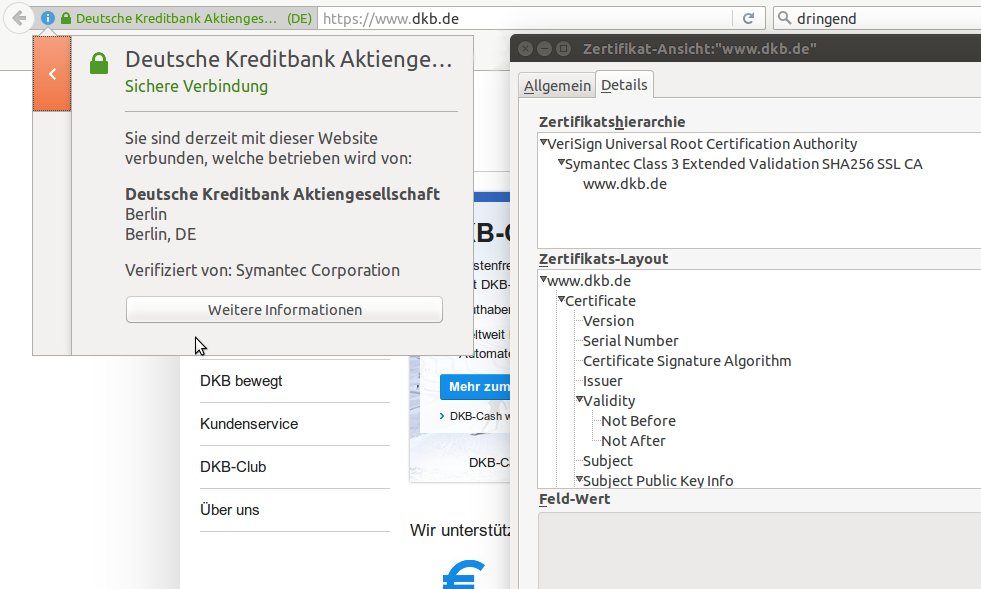
\includegraphics[width=.7\linewidth]{images/ca_dkb.png}
	\caption{Aufruf der DKB Webseite. Details des Zertifikats, welches für die Verbindung verwendet wird}
\end{figure}
\noindent
Verschiedene Webseiten, z. B. \url{https://globalsign.ssllabs.com}, bieten eine Überprüfung der gewünschten Webseite an. Als Ergebnis zeigen sie unter anderem an, welches originale Zertifikat diese Webseite wirklich verwendet. Mittels dieser Information und der Zertifikats-Eigenschaften durch den Browser ist jeder Internetnutzer in der Lage zu vergleichen, ob die verschlüsselte Verbindung das richtige Zertifikat nutzt. Handelt es sich nicht um das korrekte, originale Zertifikat und gab es zusätzlich keine Fehlermeldung/Warnung, so muss davon ausgegangen werden, dass keine direkte Verbindung zu der gewünschten Webseite besteht. Solche Fälle deuten stark darauf hin, dass die verschlüsselte Verbindung durch eine MITM-Attacke aufgebrochen wurde und die Daten eventuell mitgelesen oder sogar manipuliert werden. Nach Aufdeckung einer solchen Attacke muss das gefälschte Zertifikat im System (Zertifikatsspeichern) gesucht und anschließend gelöscht werden. Dabei ist zu beachten, dass es nicht immer ausreicht nur das entdeckte Zertifikat selbst zu löschen. Da Zertifikate auf der Basis einer Public Key Infrastruktur \cite[vgl.]{x.509} erstellt sind, können noch weitere Zertifikate für solch eine Attacke verantwortlich sein. Es sollten, neben dem aufgespürten, gefälschten Zertifikat, zusätzlich alle anderen Zertifikate, die sich in der hierarchischen Kette befinden, überprüft und ggf. entfernt werden. Im Lenovo-Beispiel konnten mittels des gehackten, selbst signierten Root-Zertifikats weitere Zertifikate erstellt werden. Mit jedem dieser Zertifikate war anschließend je eine separate MITM-Attacke möglich. Das Sicherheitsproblem war mit der Eliminierung des für die MITM Attacke verwendeten Zertifikats noch nicht gelöst. Erst nach erfolgreichem Entfernen des selbst signierten Root-Zertifikats konnten keine weiteren gefälschten Zertifikate erzeugt werden.\\
Beim DELL-Vorfall schrieb Liam Tung auf der ZDNET-Webseite: 
\begin{quote}
	\glqq [...] das einfache Entfernen des eDELLRoot-Zertifikats aus dem Administrator und persönlichen Zertifikatsspeicher ist nicht genug, um den Nutzer zu schützen. Einige Nutzer haben in der Tat berichtet, dass das Zertifikat nach einem Neustart wieder aufgetaucht ist.\grqq \cite{zdnet}	
\end{quote}
Ursache für die Neuinstallation ist das DELL-Programm „Dell Foundation Services“, welches dieses Zertifikat verwendet. Erst mit der Deinstallation des Programms bzw. eines Plug-ins des Programms und der manuellen Löschung des DELL Zertifikats ist das selbst signierte Zertifikat dauerhaft vom System erfolgreich entfernt und die Sicherheitslücke geschlossen worden. Liam Tung schrieb zur korrekten Entfernung: 
\begin{quote}
	\glqq Um es dauerhaft zu entfernen und um zu verhindern, dass es sich erneut installiert, müssen Nutzer das eDELL Plugin entfernen.\grqq \cite{zdnet}
\end{quote}
Für die detaillierte Information um welches Plug-in es sich genau handelt und worauf besonders zu achten ist, nutzt er die Ergebnisse von den Duo Security Forschern Darren Kemp, Michail Davidov und Kyle Lady.
\begin{quote}
	\glqq‘Dies kann vollbracht werden mit Hilfe der Löschung des \newline Dell.Foundation.Agent.Plugins.eDell.dll Moduls vom System. Geschieht dies nicht, so kann es weiterhin zur Aussetzung dieser Sicherheitslücke kommen.‘, sagte Duo Security.
	\\
	‘Beachte, immer wenn sie ein Werksreset auf ihrem DELL System durchführen, wird dieses Zertifikat und das eDell Plugin auf dem System wieder hergestellt und sie müssen es erneut manuell entfernen‘ [...]\grqq \cite{zdnet}
\end{quote}
Die beiden Beispiele zeigen, dass es nicht ausreicht nur die Zertifikatsspeicher auf ungewöhnliche Eintragungen zu durchsuchen, sondern ebenfalls die Programmliste des Systems auf unerwartete oder ggf. unnötig installierte Programme zu kontrollieren.
%\\
%Neben den Anwendern (Clients) könnten auch die Webserver, die die Internetseiten zur Verfügung stellen, gegen MITM-Attacken vorbeugen. %Das SSL Protocol unterstützt nicht nur eine Server-seitige Authentifizierung sonder auch eine Client-seitige Authentifizierung. Durch %solch eine zweiseitige Authentifizierung wird eine MITM-Attacke erschwert. Problem dabei ist die hohe Anzahl an Clients und die dafür %benötigten individuellen Client-Zertifikate. Diese Zertifikate müssten am besten von öffentlichen Zertifizierungsstellen ausgestellt %werden, damit die Server nicht jedes Client-Zertifikat extra in ihren Zertifikatsspeicher aufnehmen müssen. Vorteil ist, dass beide %Seiten ihre Identität nachweisen müssen und somit eine doppelte Überprüfung der Kommunikationspartner stattfindet.